\chapter{Results}
\label{ch:results}

In this chapter, we first describe our evaluation setup, which consists of the HPC cluster used for our experiments, the matrix datasets, and the algorithmic implementations evaluated. We then present a detailed analysis of various performance metrics, including execution time, memory usage, parallelization and matrix fill-in reduction. 


% In this chapter, you want to show that your implementation meets the objectives.
% Start by briefly describing the type of results you have collected and how these results relate to the objectives.

\section{Evaluation setup}

Everything that is evaluated is ran on Fritz, a high-performance computing cluster at NHR@FAU.

\subsection{Hardware Infrastructure}

Fritz is a parallel CPU cluster operated by NHR@FAU, featuring Intel Ice Lake and Sapphire Rapids processors with an InfiniBand (IB) network and a Lustre-based parallel filesystem accessible under \texttt{\$FASTTMP}. The cluster configuration consists of:
\begin{table}[h]
\centering
\begin{tabular}{|p{1.5cm}|p{4.5cm}|p{2cm}|p{3cm}|}
\hline
\textbf{Nodes} & \textbf{CPUs and Cores} & \textbf{Memory} & \textbf{Slurm Partition} \\
\hline
992 & 2 × Intel Xeon Platinum 8360Y (Ice Lake) & 256 GB & singlenode, multinode \\
  & 2 × 36 cores @2.4 GHz & & \\
\hline
48 & 2 × Intel Xeon Platinum 8470 (Sapphire Rapids) & 1 TB & spr1tb \\
   & 2 × 52 cores @2.0 GHz & & \\
\hline
16 & 2 × Intel Xeon Platinum 8470 (Sapphire Rapids) & 2 TB & spr2tb \\
   & 2 × 52 cores @2.0 GHz & & \\
\hline
\end{tabular}
\caption{Fritz cluster node configuration}
\label{tab:fritz-nodes}
\end{table}

The login nodes fritz[1-4] are equipped with 2 × Intel Xeon Platinum 8360Y (Ice Lake) processors and 512 GB main memory. Additionally, the remote visualization node fviz1 features 2 × Intel Xeon Platinum 8360Y processors with 1 TB main memory, one Nvidia A16 GPU, and 30 TB of local NVMe SSD storage.



% Precisely describe your measurement/evaluation setup in a top-down manner.
% For example:
% \begin{itemize}
%   \item If you used a development platform, which one and how was it configured?
%   \item Which tools did you use?
%   \item What input data set / program / signals / \ldots{} did you use?
%     If your data set is very large, you should fully define and describe it in an appendix chapter and refer to that definition here using simple labels.
%   \item If your implementation is configurable, which configuration(s) did you evaluate?
% \end{itemize}

% The information given here (with references to external work) should be sufficient to reproduce the setup you used for your measurements.

\section{Matrices dataset}

We selected a diverse set of sparse matrices from the SuiteSparse Matrix Collection and our custom dataset of matrices encountered in Quantum Transport to evaluate our implementations. The SuiteSparse matrices chosen are usually which were commonly used in the literature for \textit{METIS} and \textit{SCOTCH} own evaluations. 
[TODO about Quantum transport matrices]

\begin{table}[h]
\centering
\caption{SuiteSparse matrix dataset used for evaluation}
\label{tab:matrix-dataset}
\resizebox{\textwidth}{!}{%
\begin{tabular}{|l|r|r|l|}
\hline
\textbf{Graph name} & \textbf{No. of vertices} & \textbf{No. of edges} & \textbf{Description} \\
\hline
144 & 144649 & 1074393 & 3D Finite element mesh \\
598A & 110971 & 741934 & 3D Finite element mesh \\
ADD32 & 4960 & 9462 & 32-bit adder \\
AUTO & 448695 & 3314611 & 3D Finite element mesh \\
BBMAT & 38744 & 99341 & 2D Stiffness matrix \\
BCSSTK30 & 28294 & 1007284 & 3D Stiffness matrix \\
BCSSTK31 & 35588 & 572914 & 3D Stiffness matrix \\
BCSSTK32 & 44609 & 985046 & 3D Stiffness matrix \\
BRACK2 & 62631 & 366559 & 3D Finite element mesh \\
CANT & 54195 & 1960797 & 3D Stiffness matrix \\
COPTER2 & 55476 & 352238 & 3D Finite element mesh \\
FINAN512 & 74752 & 261120 & Linear programming \\
LHR10 & 10672 & 209093 & Chemical engineering \\
LHR71 & 70304 & 1449248 & Chemical engineering \\
M14B & 214765 & 3358036 & 3D Finite element mesh \\
MEMPLUS & 17758 & 54196 & Memory circuit \\
PWT & 36519 & 144793 & 3D Finite element mesh \\
SHYY161 & 76480 & 152002 & CFD/Navier-Stokes \\
TORSO1 & 201142 & 1479989 & 3D Finite element mesh \\
TROLL & 213453 & 5858829 & 3D Stiffness matrix \\
VENKAT01 & 62424 & 827684 & 2D Coefficient matrix \\
WAVE & 156317 & 1059331 & 3D Finite element mesh \\
\hline
\end{tabular}%
}
\end{table}

\begin{table}[h]
\centering
\caption{Quantum Transport matrix dataset used for evaluation}
\label{tab:qt-matrix-dataset}
\resizebox{\textwidth}{!}{%
\begin{tabular}{|l|r|r|l|}
\hline
\textbf{Graph name} & \textbf{No. of vertices} & \textbf{No. of edges} & \textbf{Description} \\
\hline
airpoll\_conditional\_st3 & 8499 & 1218651 & Spatio-temporal statistical Modelling \\
airpoll\_prior\_st3 & 8499 & 1205931 & Spatio-temporal statistical Modelling \\
cnt\_cp2k & 9152 & 6154350 & DFT Hamiltonian of Carbon Nanotube \\
cnt\_w90 & 768 & 71680 & DFT Hamiltonian of Carbon Nanotube \\
kmc\_potential\_0 & 403605 & 10007089 & Kinetic Monte Carlo for Device Modelling \\
kmc\_potential\_1 & 1632355 & 41208963 & Kinetic Monte Carlo for Device Modelling \\
qubit\_fem\_b4 & 116380 & 2517228 & FEM Matrix for Qubit \\
sinw\_w90 & 7488 & 5310160 & DFT Hamiltonian of Silicon Nanowire \\
\hline
\end{tabular}%
}
\end{table}

\section{Methodology}

For our evaluation, we systematically assessed the performance of eleven different reordering algorithms across all matrices listed in Tables~\ref{tab:matrix-dataset} and~\ref{tab:qt-matrix-dataset}. The evaluated algorithms encompass both sequential and parallel approaches, ranging from classical degree-based methods to graph partitioning and hypergraph-based techniques:

\begin{description}
   \item[\textbf{Classical Methods:}] \mbox{}\\
   \begin{itemize}
      \item \textbf{AMD} -- Approximate Minimum Degree
      \item \textbf{COLAMD} -- Column Approximate Minimum Degree  
      \item \textbf{RCM} -- Reverse Cuthill-McKee
      \item \textbf{Natural} -- Original matrix ordering (baseline)
   \end{itemize}
   
   \item[\textbf{Graph Partitioning Methods:}] \mbox{}\\
   \begin{itemize}
      \item \textbf{METIS} -- Sequential graph partitioning-based reordering
      \item \textbf{METIS+IC} -- METIS with improved coarsening integration
      \item \textbf{SCOTCH} -- Sequential graph partitioning
      \item \textbf{PT-SCOTCH} -- Parallel graph partitioning
      \item \textbf{ParMETIS} -- Parallel graph partitioning
   \end{itemize}
   
   \item[\textbf{Hypergraph-based Methods:}] \mbox{}\\
   \begin{itemize}
      \item \textbf{HG-2, HG-4, HG-8, HG-16} -- Hypergraph-based reordering with block partition sizes of 2, 4, 8, and 16 vertices respectively
   \end{itemize}
\end{description}

The hypergraph-based methods (HG-2, HG-4, HG-8, HG-16) employ different block partition sizes to explore the trade-off between computational complexity and reordering/parallelization quality. All these algorithms are described in detail in Chapter~\ref{ch:background}.

\subsection{Performance Metrics and Measurement Protocol}

Our comprehensive evaluation measures five key performance indicators to assess the effectiveness of each reordering algorithm:

\begin{description}
   \item[\textbf{Fill-in Reduction:}] We measure the number of non-zero entries introduced during symbolic Cholesky factorization using the \texttt{cmpfillin} binary provided by the METIS library. This tool performs symbolic factorization (as described in Chapter~\ref{ch:background}) to count the additional non-zero entries without executing the actual numerical computation. 
      
      \item[\textbf{Computational Complexity:}] We track the total floating-point operation count required for factorization, providing insight into the computational efficiency gains achieved by different reordering strategies.
      
      \item[\textbf{Reordering Time:}] The wall-clock time required to compute the reordering itself is measured using Python's \texttt{time.perf\_counter()} with microsecond precision. This overhead cost is crucial for understanding the practical applicability of each method.
      
      \item[\textbf{Memory Usage:}] We implement a dedicated memory monitoring system using a separate thread that samples memory consumption every 50 milliseconds during reordering operations. The monitoring captures both peak memory usage (maximum RSS observed) and average memory consumption throughout the reordering process. Memory measurements are obtained via the \texttt{psutil} library, tracking the resident set size (RSS) of the process and computing the memory increase relative to a baseline measured before algorithm execution.

      \item[\textbf{Parallelization Potential:}] We assess the elimination tree depth as an indicator of the inherent parallelism available in the factorization. As mentioned in Chapter~\ref{ch:background}, the elimination tree is constructed by identifying parent-child relationships in the symbolic factorization structure, where the tree depth represents the critical path length and thus the theoretical lower bound on parallel factorization time.
\end{description}

For memory profiling, we initially attempted to use the Massif profiler from Valgrind, but encountered issues with our Python-based implementations and the cluster environment. Consequently, we developed a custom memory measurement protocol that employs a thread-safe monitoring system to capture accurate memory usage patterns during reordering operations.

Our memory measurement implementation works by first establishing a baseline memory consumption before starting any reordering algorithm, recording the initial resident set size (RSS) using \texttt{psutil.Process().memory\_info().rss}. During algorithm execution, a dedicated monitoring thread runs concurrently, sampling memory usage every 50 milliseconds throughout the entire operation. This thread continuously updates the maximum observed memory consumption and maintains a comprehensive list of all samples for subsequent average computation.

Upon completion of the reordering algorithm, we compute both the peak memory increase (calculated as the maximum observed RSS minus the baseline) and the average memory increase (computed as the mean of all samples minus the baseline), with results reported in kilobytes. For cases where the monitoring thread fails to capture meaningful data, such as very fast operations that complete before sufficient samples can be collected, we provide conservative estimates based on matrix characteristics, using approximately 10\% of the matrix storage size as an upper bound for memory consumption.

All experiments are executed on the Fritz cluster to ensure consistent hardware conditions across all measurements. Each algorithm is tested on every matrix in our dataset, and results are averaged over five independent runs to mitigate variability. 

\section{Evaluation}

For each matrix in our dataset with different reordering algorithms applied, we have collected all the aforementioned metrics, and these can be found in our appendix/supplementary material \ref{app:experimental_results}. Here, we present results and visualizations for our underlying metrics for some of them.

Figure~\ref{fig:fill-in-comparison} presents a comparative analysis of fill-in reduction performance across our key reordering algorithms for a representative subset of matrices from our dataset. The results are normalized relative to AMD performance to facilitate direct comparison across different matrix types and sizes.
\begin{figure}[H]
\centering
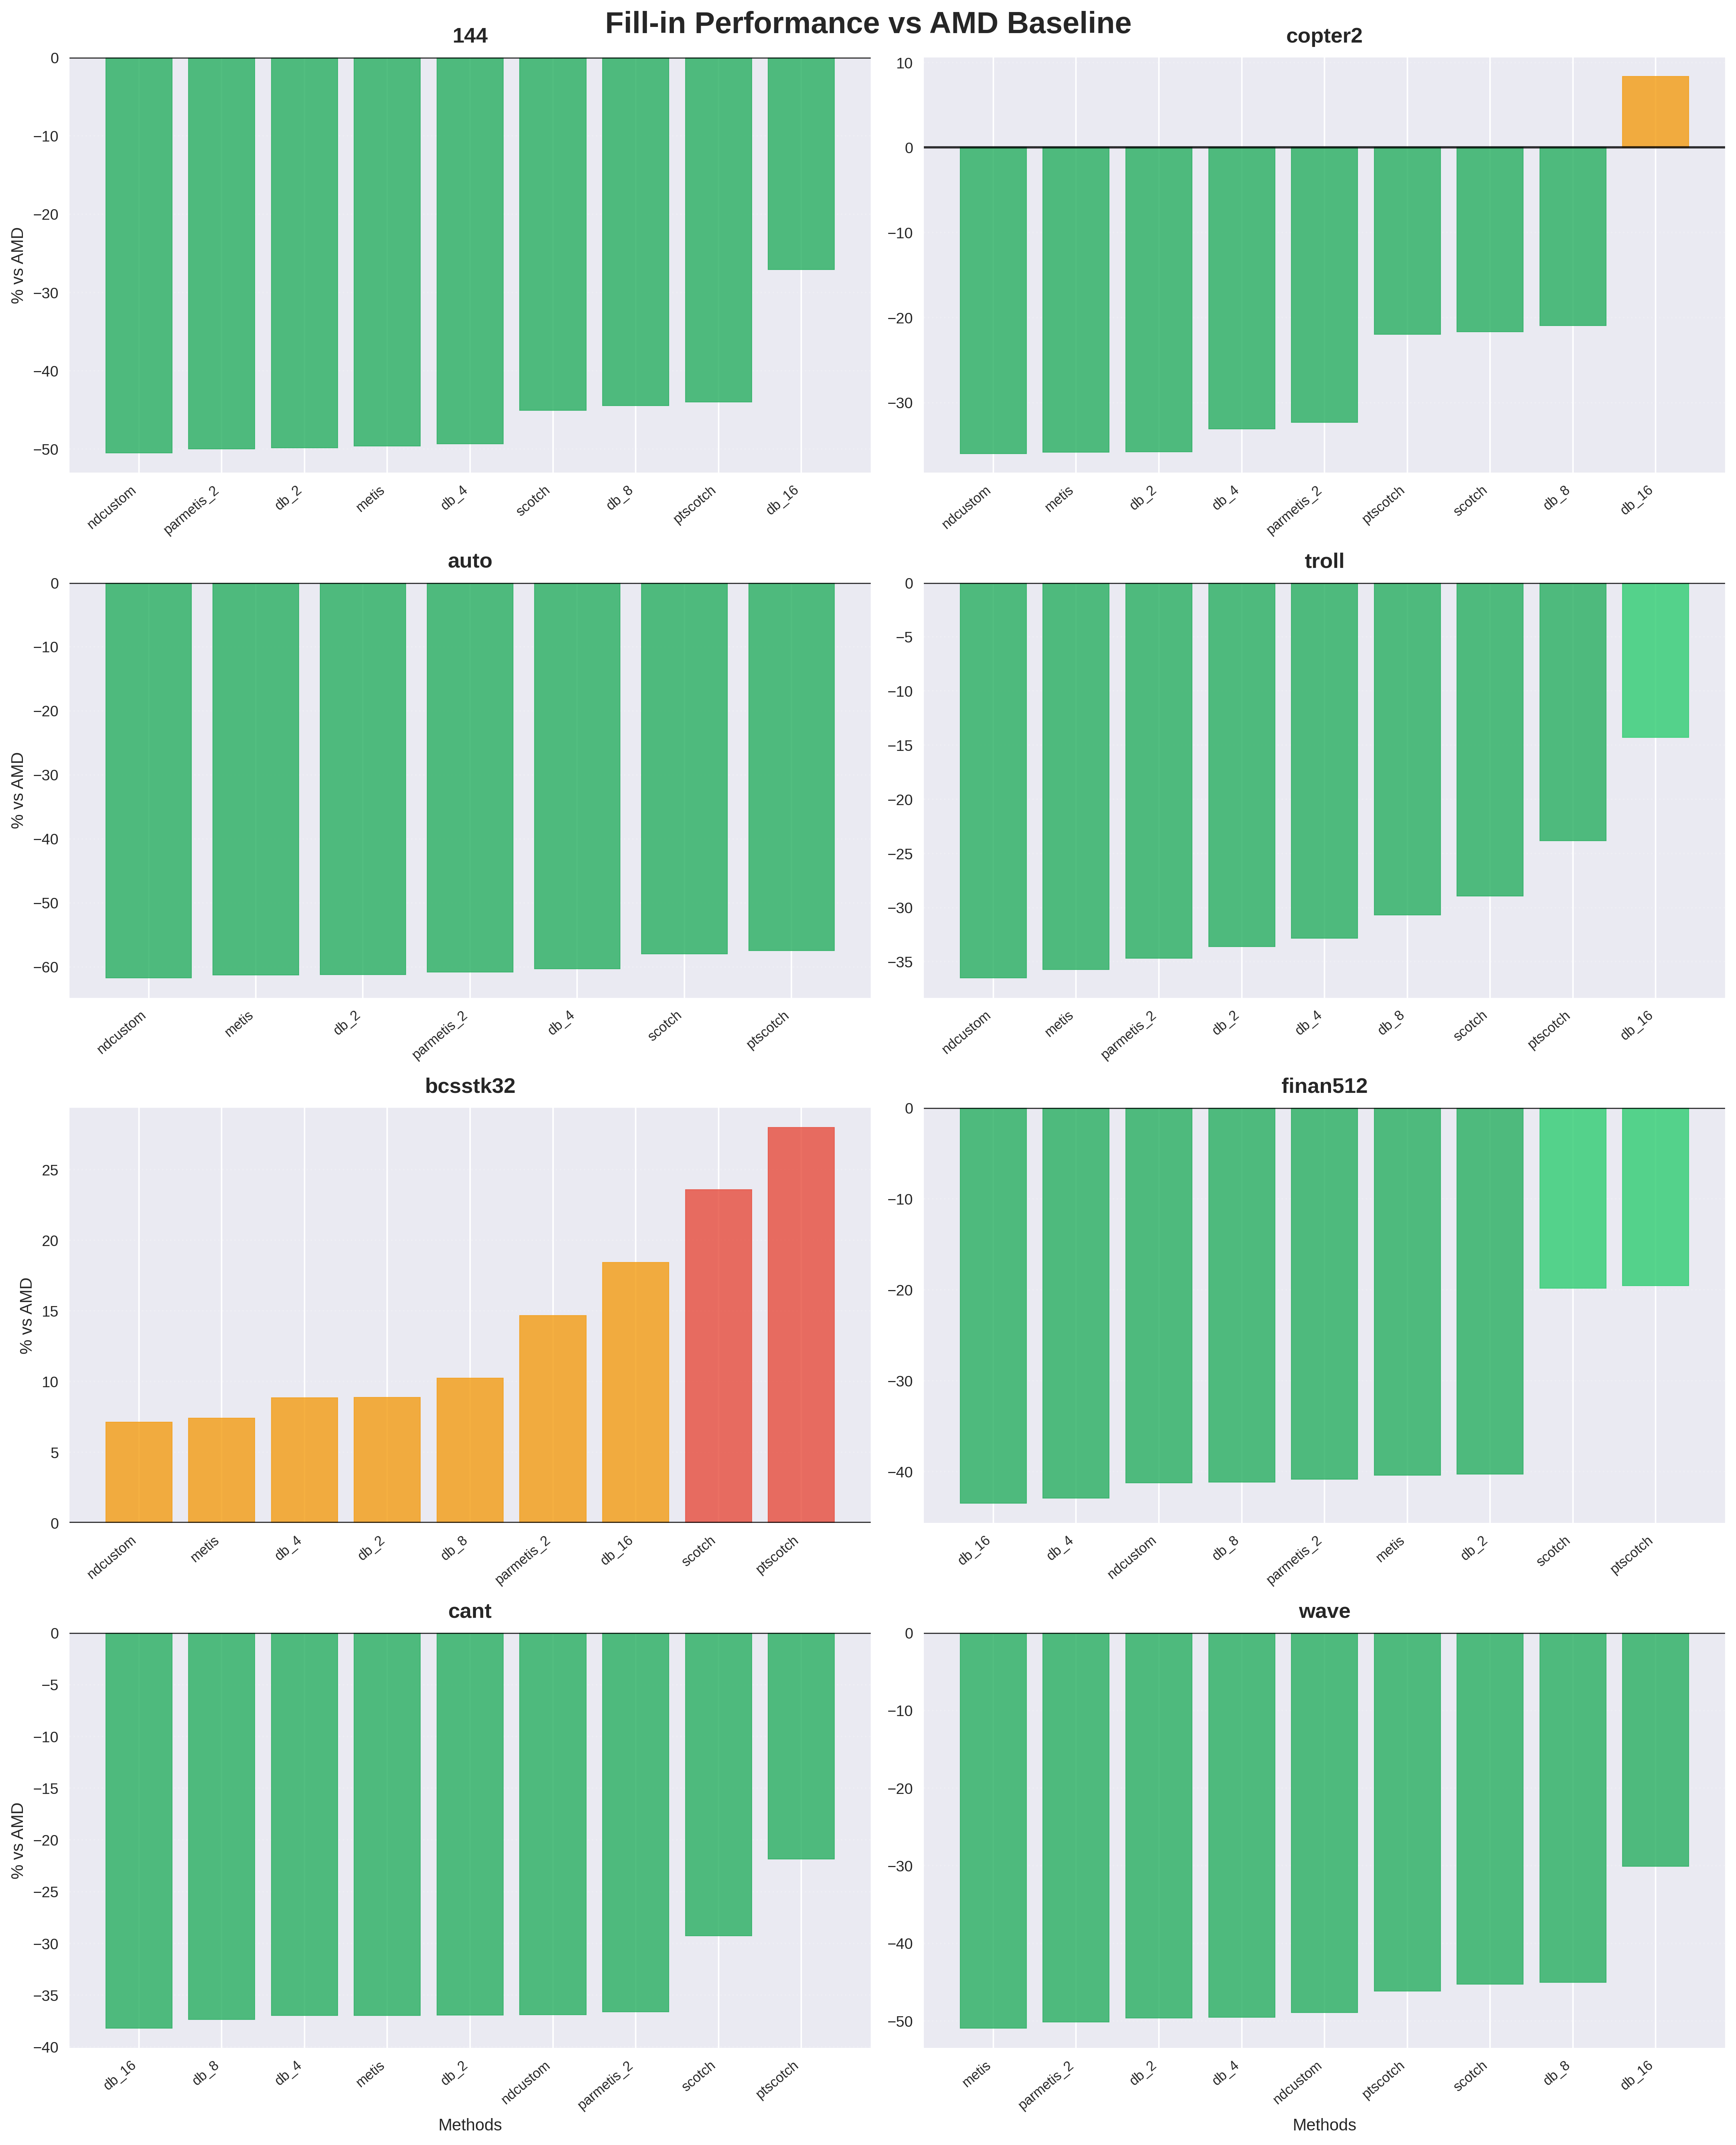
\includegraphics[width=\textwidth]{fig/res/fill-in-comp.png}
\caption{Fill-in reduction comparison across reordering algorithms for selected matrices. Results are shown as percentages relative to AMD performance. Methods with exceptionally high fill-in (RCM, Natural ordering) are excluded for clarity. ParMETIS results represent the 2-processor variant.}
\label{fig:fill-in-comparison}
\end{figure}

The sparsity pattern visualization in Figure~\ref{fig:144-sparsity-patterns} provides intuitive insight into how different reordering algorithms restructure the matrix 144. The natural ordering shows a scattered, unstructured pattern that leads to extensive fill-in during factorization. In contrast, the optimized reorderings demonstrate clear improvements in matrix structure, with methods like METIS and the hypergraph-based approaches creating more clustered patterns that minimize fill-in. Similarly, the results for matrix copter2 in Figure~\ref{fig:copter2-sparsity-patterns} reveal comparable trends.


\begin{figure}[h]
\centering
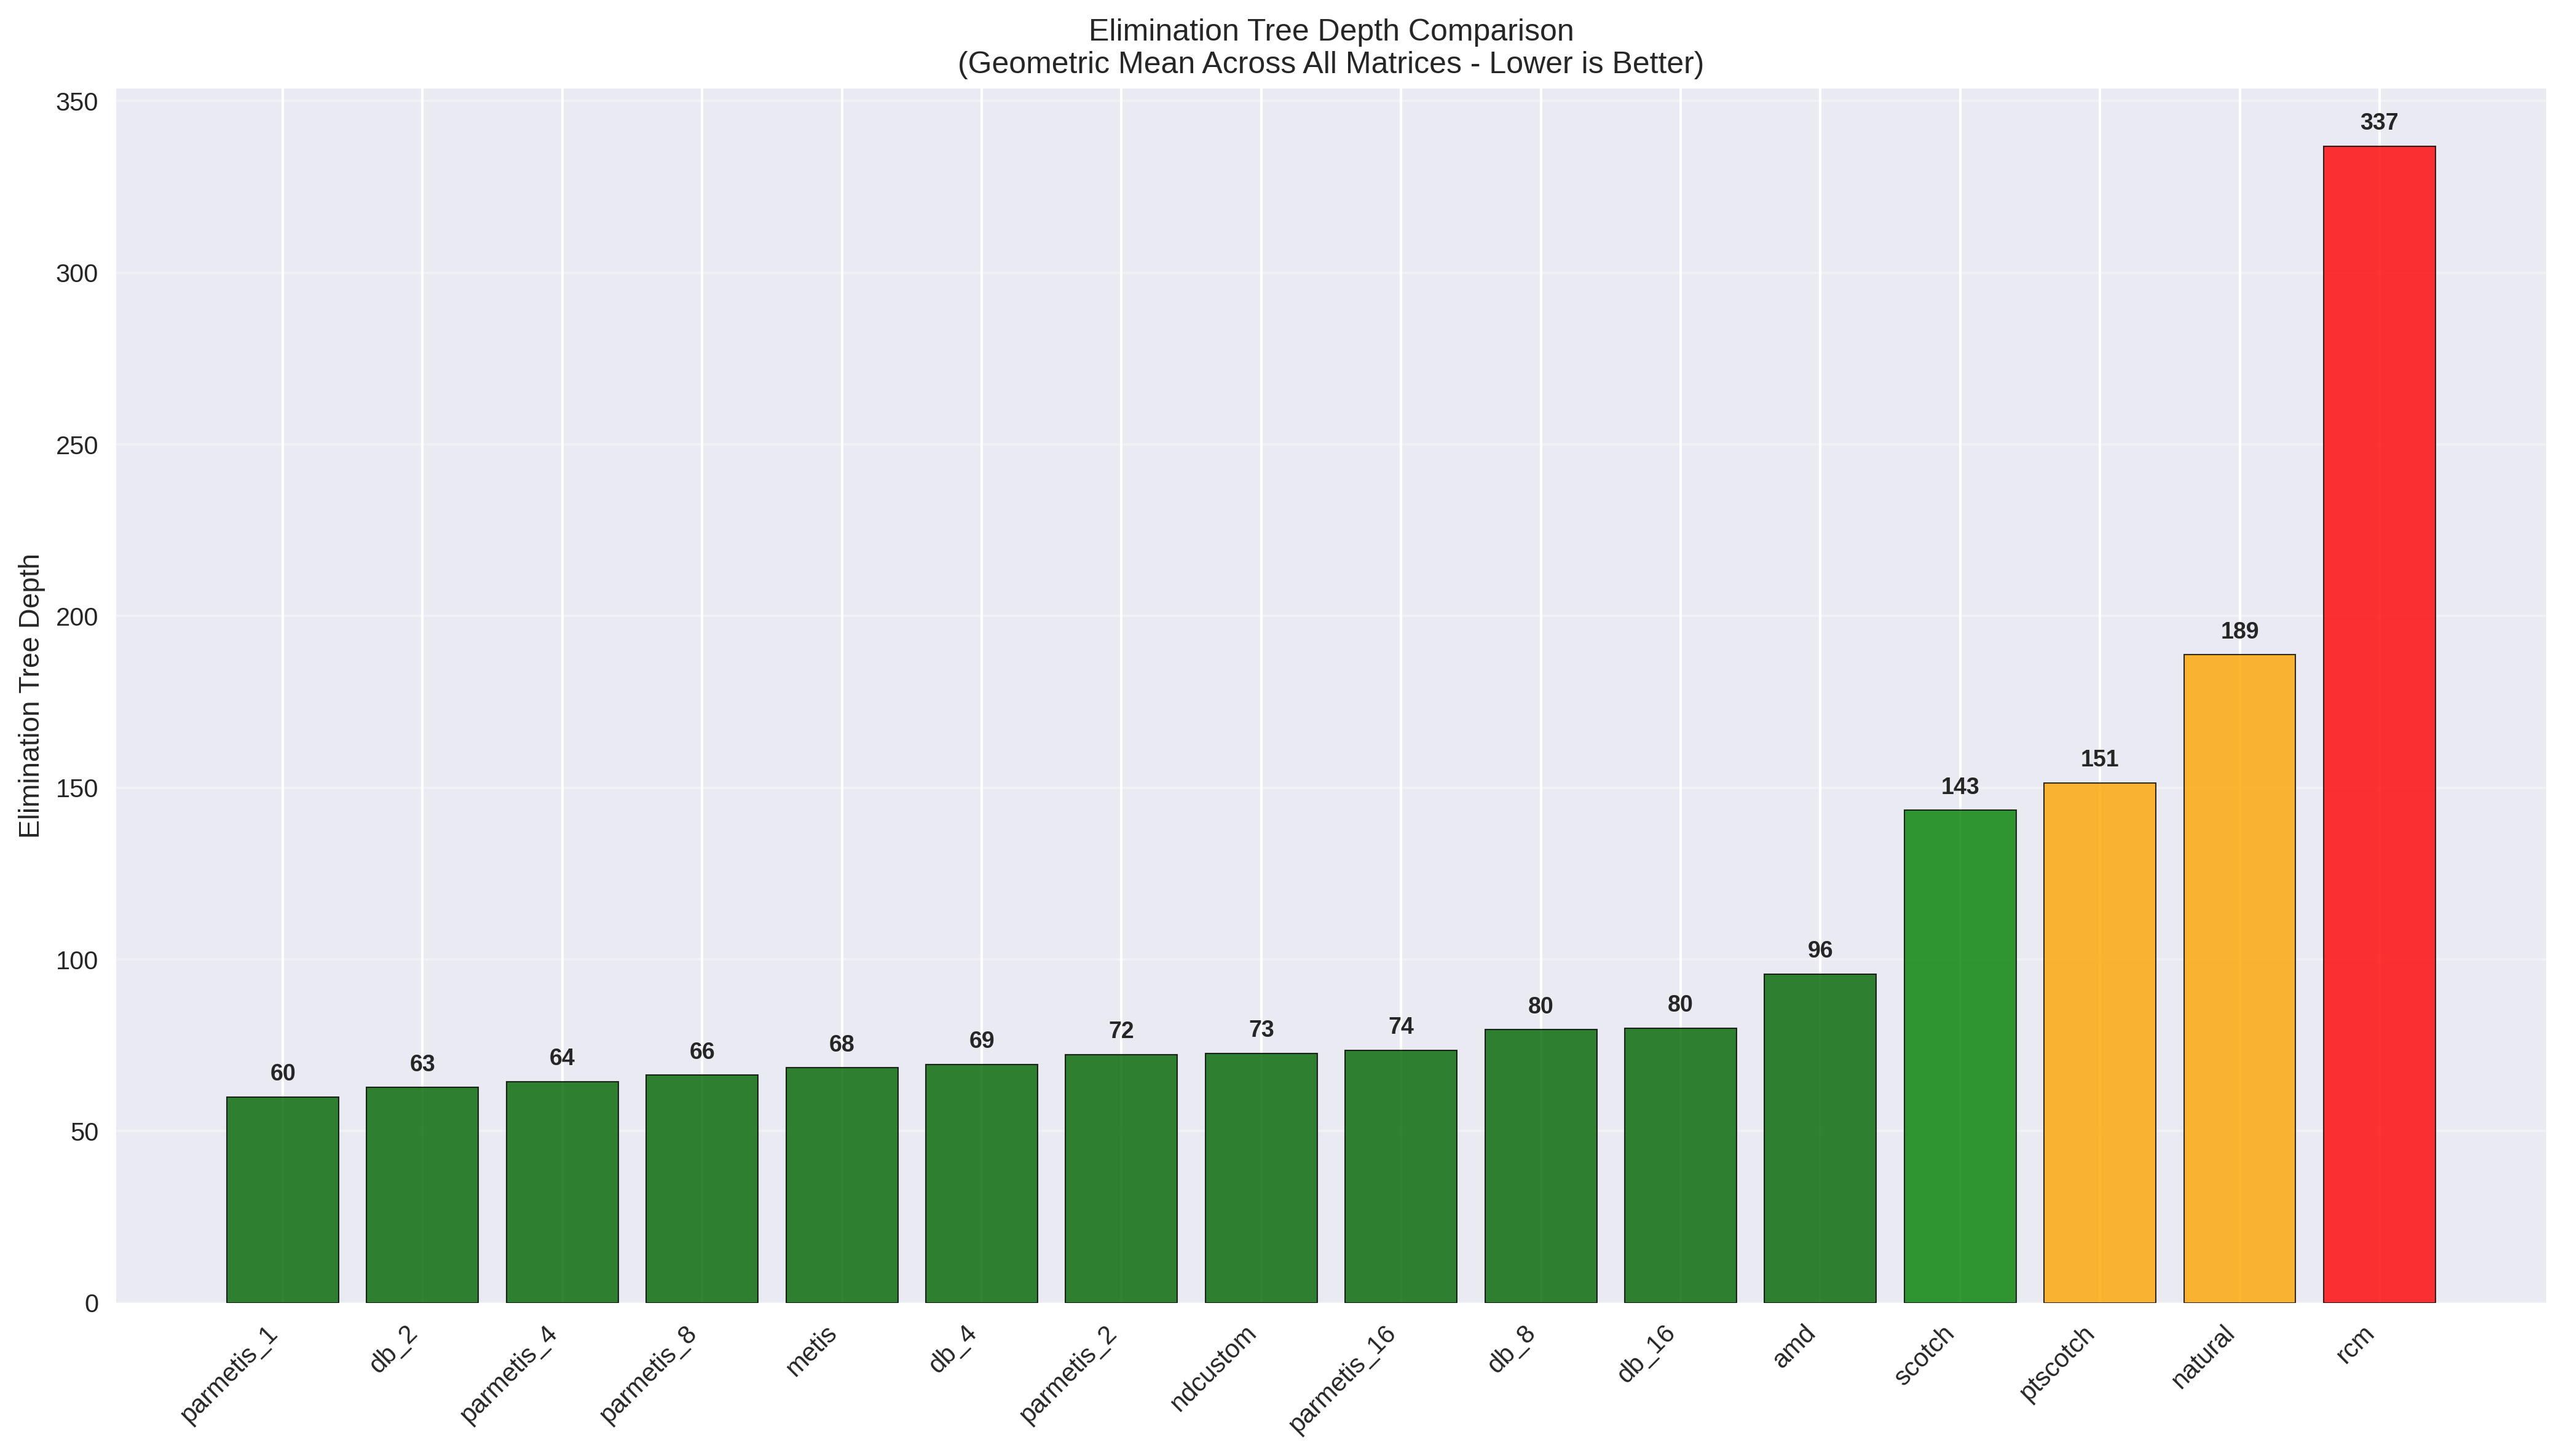
\includegraphics[width=\textwidth]{fig/res/elimination_tree_depth_comparison.png}
\caption{Elimination tree depth comparison across different reordering algorithms. The geometric mean shows the relative parallelization potential, where lower depths indicate better parallel scalability for factorization.}
\label{fig:elimination-tree-depth}
\end{figure}

The elimination tree depth analysis in Figure~\ref{fig:elimination-tree-depth} reveals the parallelization potential of each reordering method. Lower elimination tree depths indicate greater opportunities for parallel factorization, as they represent shorter critical paths in the dependency graph. 

Reordering time is another practical consideration regarding computational overhead, particularly how execution time scales with matrix size. Figure~\ref{fig:reordering-time-vs-size} illustrates the relationship between matrix size (number of vertices) and reordering time for different algorithms across our entire dataset.

\begin{figure}[h]
\centering
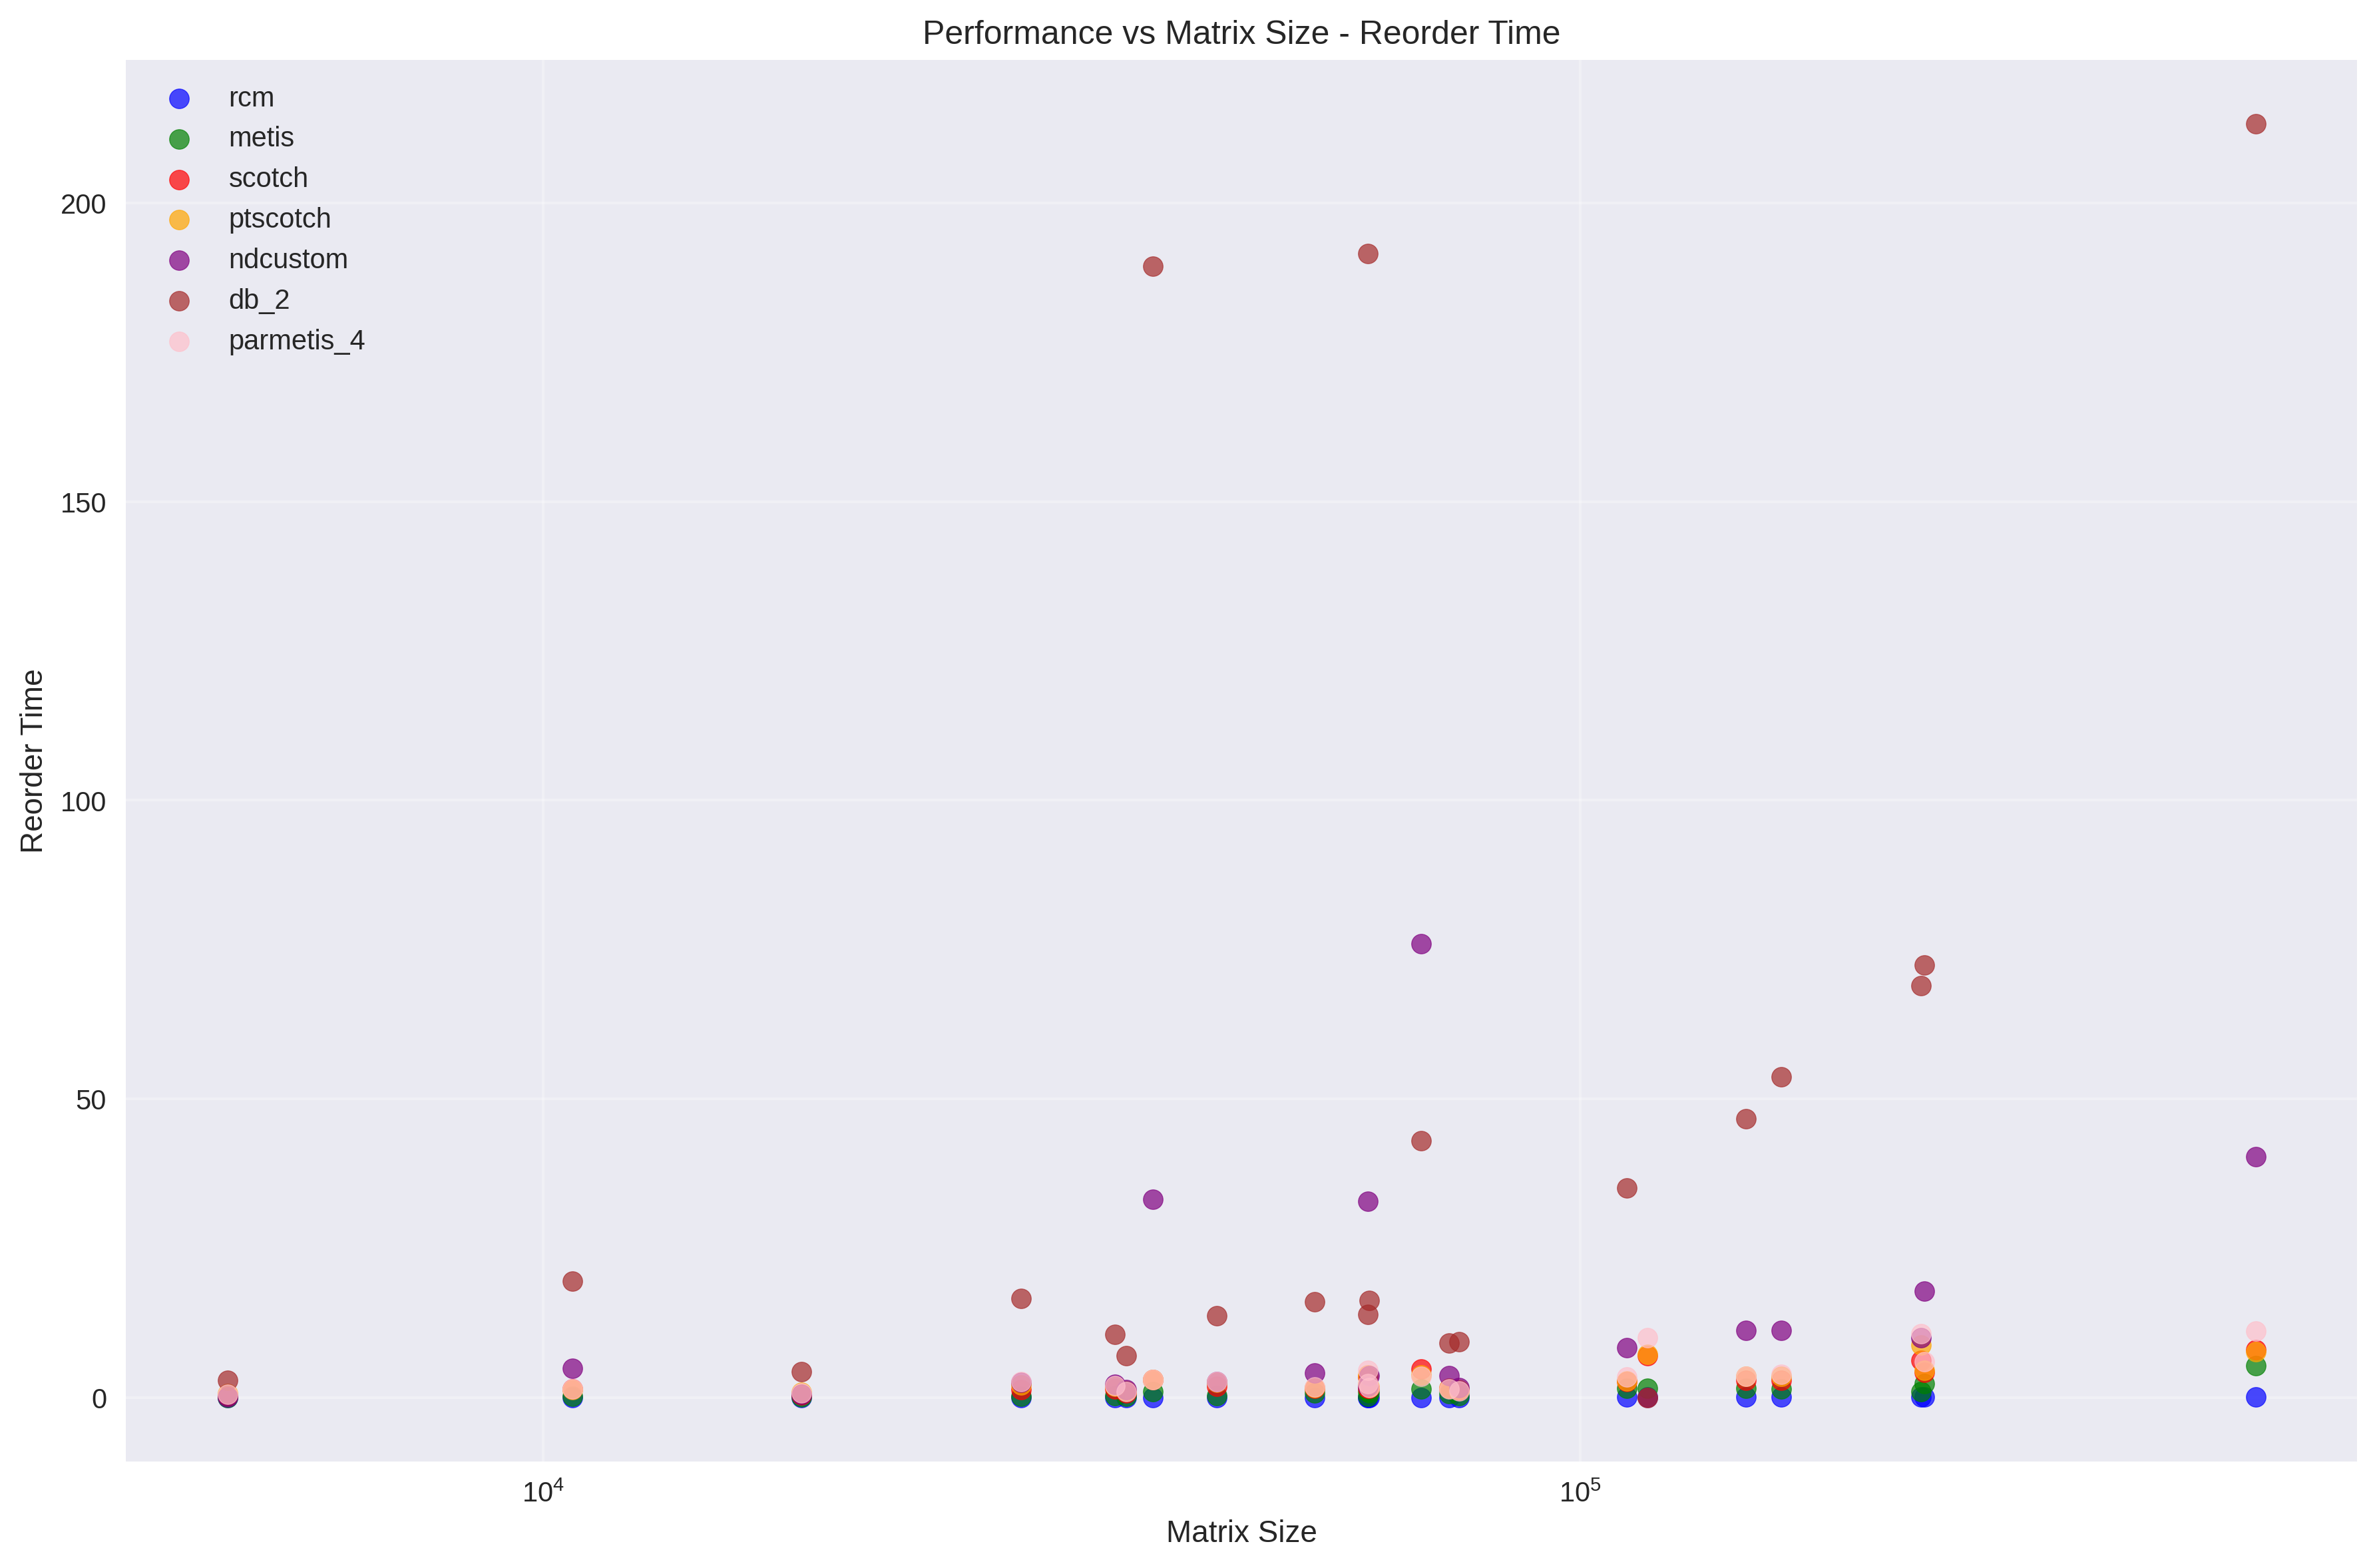
\includegraphics[width=0.8\textwidth]{fig/res/reorder_time_vs_size.png}
\caption{Reordering time as a function of matrix size for different algorithms}
\label{fig:reordering-time-vs-size}
\end{figure}

The performance analysis reveals distinct computational overhead characteristics across different algorithm categories. AMD and RCM are the fastest methods, benefiting from their simple computational kernels. Among nested dissection approaches, METIS is the fastest, while ParMETIS and PT-SCOTCH are slower, likely due to parallelization overhead that outweighs benefits for our matrix sizes. The hypergraph methods (HG-2, HG-4, HG-8, HG-16) were considerably the slowest by far, due to the inherent complexity of hypergraph partitioning algorithms involving multiple coarsening, partitioning, and refinement phases.

% \subsection{Fill-in Analysis}

% Table~\ref{tab:fillin-results} presents the fill-in results for all evaluated reordering algorithms across our matrix dataset. Fill-in represents the number of additional non-zero entries introduced during Cholesky factorization, which directly impacts both memory requirements and computational complexity.

\begin{table}[h]
\centering
\caption{Fill-in results for different reordering algorithms (number of non-zeros after symbolic factorization)}
\label{tab:fillin-results}
\rotatebox{90}{%
\resizebox{\textheight}{!}{%
\begin{tabular}{|l|r|r|r|r|r|r|r|r|r|r|r|}
\hline
\textbf{Matrix} & \textbf{AMD} & \textbf{COLAMD} & \textbf{HG-16} & \textbf{HG-2} & \textbf{HG-4} & \textbf{HG-8} & \textbf{METIS} & \textbf{Natural} & \textbf{METIS+IC} & \textbf{RCM} & \textbf{SCOTCH} \\
\hline
144 & 93410000 & 93410000 & 68090000 & 46850000 & 47320000 & 51880000 & 47060000 & 1.845E+19 & 46230000 & 925100000 & 51300000 \\
598a & 45810000 & 45810000 & 40670000 & 25590000 & 25870000 & 29360000 & 25480000 & - & 25460000 & - & 28370000 \\
add32 & 9417 & 9417 & 9830 & 10030 & 10120 & 10120 & 10050 & 2658000 & 9995 & 14610 & 20300 \\
auto & 569500000 & 569500000 & - & 220800000 & 226000000 & - & 220600000 & - & 217900000 & - & 243900000 \\
bbmat & 16860000 & 16860000 & 18340000 & 15780000 & 16100000 & 16370000 & 15910000 & - & 15750000 & 33750000 & 17800000 \\
bcsstk30 & 3823000 & 3823000 & 4806000 & 4354000 & 4507000 & 4345000 & 4277000 & 15690000 & 4300000 & 21110000 & 4541000 \\
bcsstk31 & 5533000 & 5533000 & 4698000 & 4248000 & 4209000 & 4313000 & 4186000 & 23140000 & 4164000 & 22400000 & 4755000 \\
bcsstk32 & 4944000 & 4944000 & 5855000 & 5383000 & 5382000 & 5451000 & 5311000 & 60770000 & 5297000 & 44020000 & 6201000 \\
brack2 & 7386000 & 7386000 & 8666000 & 5732000 & 5906000 & 6693000 & 5870000 & 759500000 & 5800000 & 45130000 & 7636000 \\
cant & 28880000 & 28880000 & 17850000 & 18210000 & 18200000 & 18090000 & 18200000 & 16780000 & 18220000 & 17150000 & 20440000 \\
copter2 & 13880000 & 13880000 & 15040000 & 8914000 & 9284000 & 10970000 & 8906000 & 702700000 & 8880000 & 68550000 & 10830000 \\
finan512 & 2763000 & 2763000 & 1562000 & 1650000 & 1577000 & 1626000 & 1647000 & 6190000 & 1623000 & 7511000 & 2197000 \\
lhr10 & 8078000 & 8078000 & 7500000 & 3130000 & 3858000 & 5469000 & 3469000 & - & 3323000 & 14980000 & 3937000 \\
lhr71 & 93700000 & 93700000 & 210300000 & 36470000 & 36060000 & 35450000 & 36040000 & 210300000 & 34550000 & 150100000 & 41460000 \\
m14b & 110300000 & 110300000 & 95120000 & 62320000 & 63220000 & 70130000 & 62610000 & - & 62130000 & - & 68790000 \\
memplus & 52430 & 52430 & 57320 & 55730 & 54660 & 55180 & 54780 & 138400000 & 55830 & 142700 & 127300 \\
pwt & 1519000 & 1519000 & 1320000 & 1307000 & 1313000 & 1319000 & 1306000 & 3396000 & 1309000 & 5362000 & 1601000 \\
shyy161 & 1746000 & 1746000 & 1653000 & 1692000 & 1639000 & 1660000 & 1657000 & 8141000 & 1672000 & 11110000 & 2042000 \\
torso1 & 12450000 & 12450000 & - & - & - & - & 13570000 & - & - & 113500000 & 16560000 \\
troll & 91680000 & 91680000 & 78570000 & 60850000 & 61560000 & 63540000 & 58910000 & 913600000 & 58210000 & 941600000 & 67080000 \\
venkat01 & 5739000 & 5739000 & 5797000 & 5378000 & 5378000 & 5472000 & 5405000 & 64940000 & 5349000 & 45380000 & 5954000 \\
wave & 121700000 & 121700000 & 85080000 & 61300000 & 61410000 & 66910000 & 59710000 & 1008000000 & 62180000 & 835800000 & 66530000 \\
\hline
\end{tabular}%
}%
}
\end{table}

\begin{figure}[h]
\centering
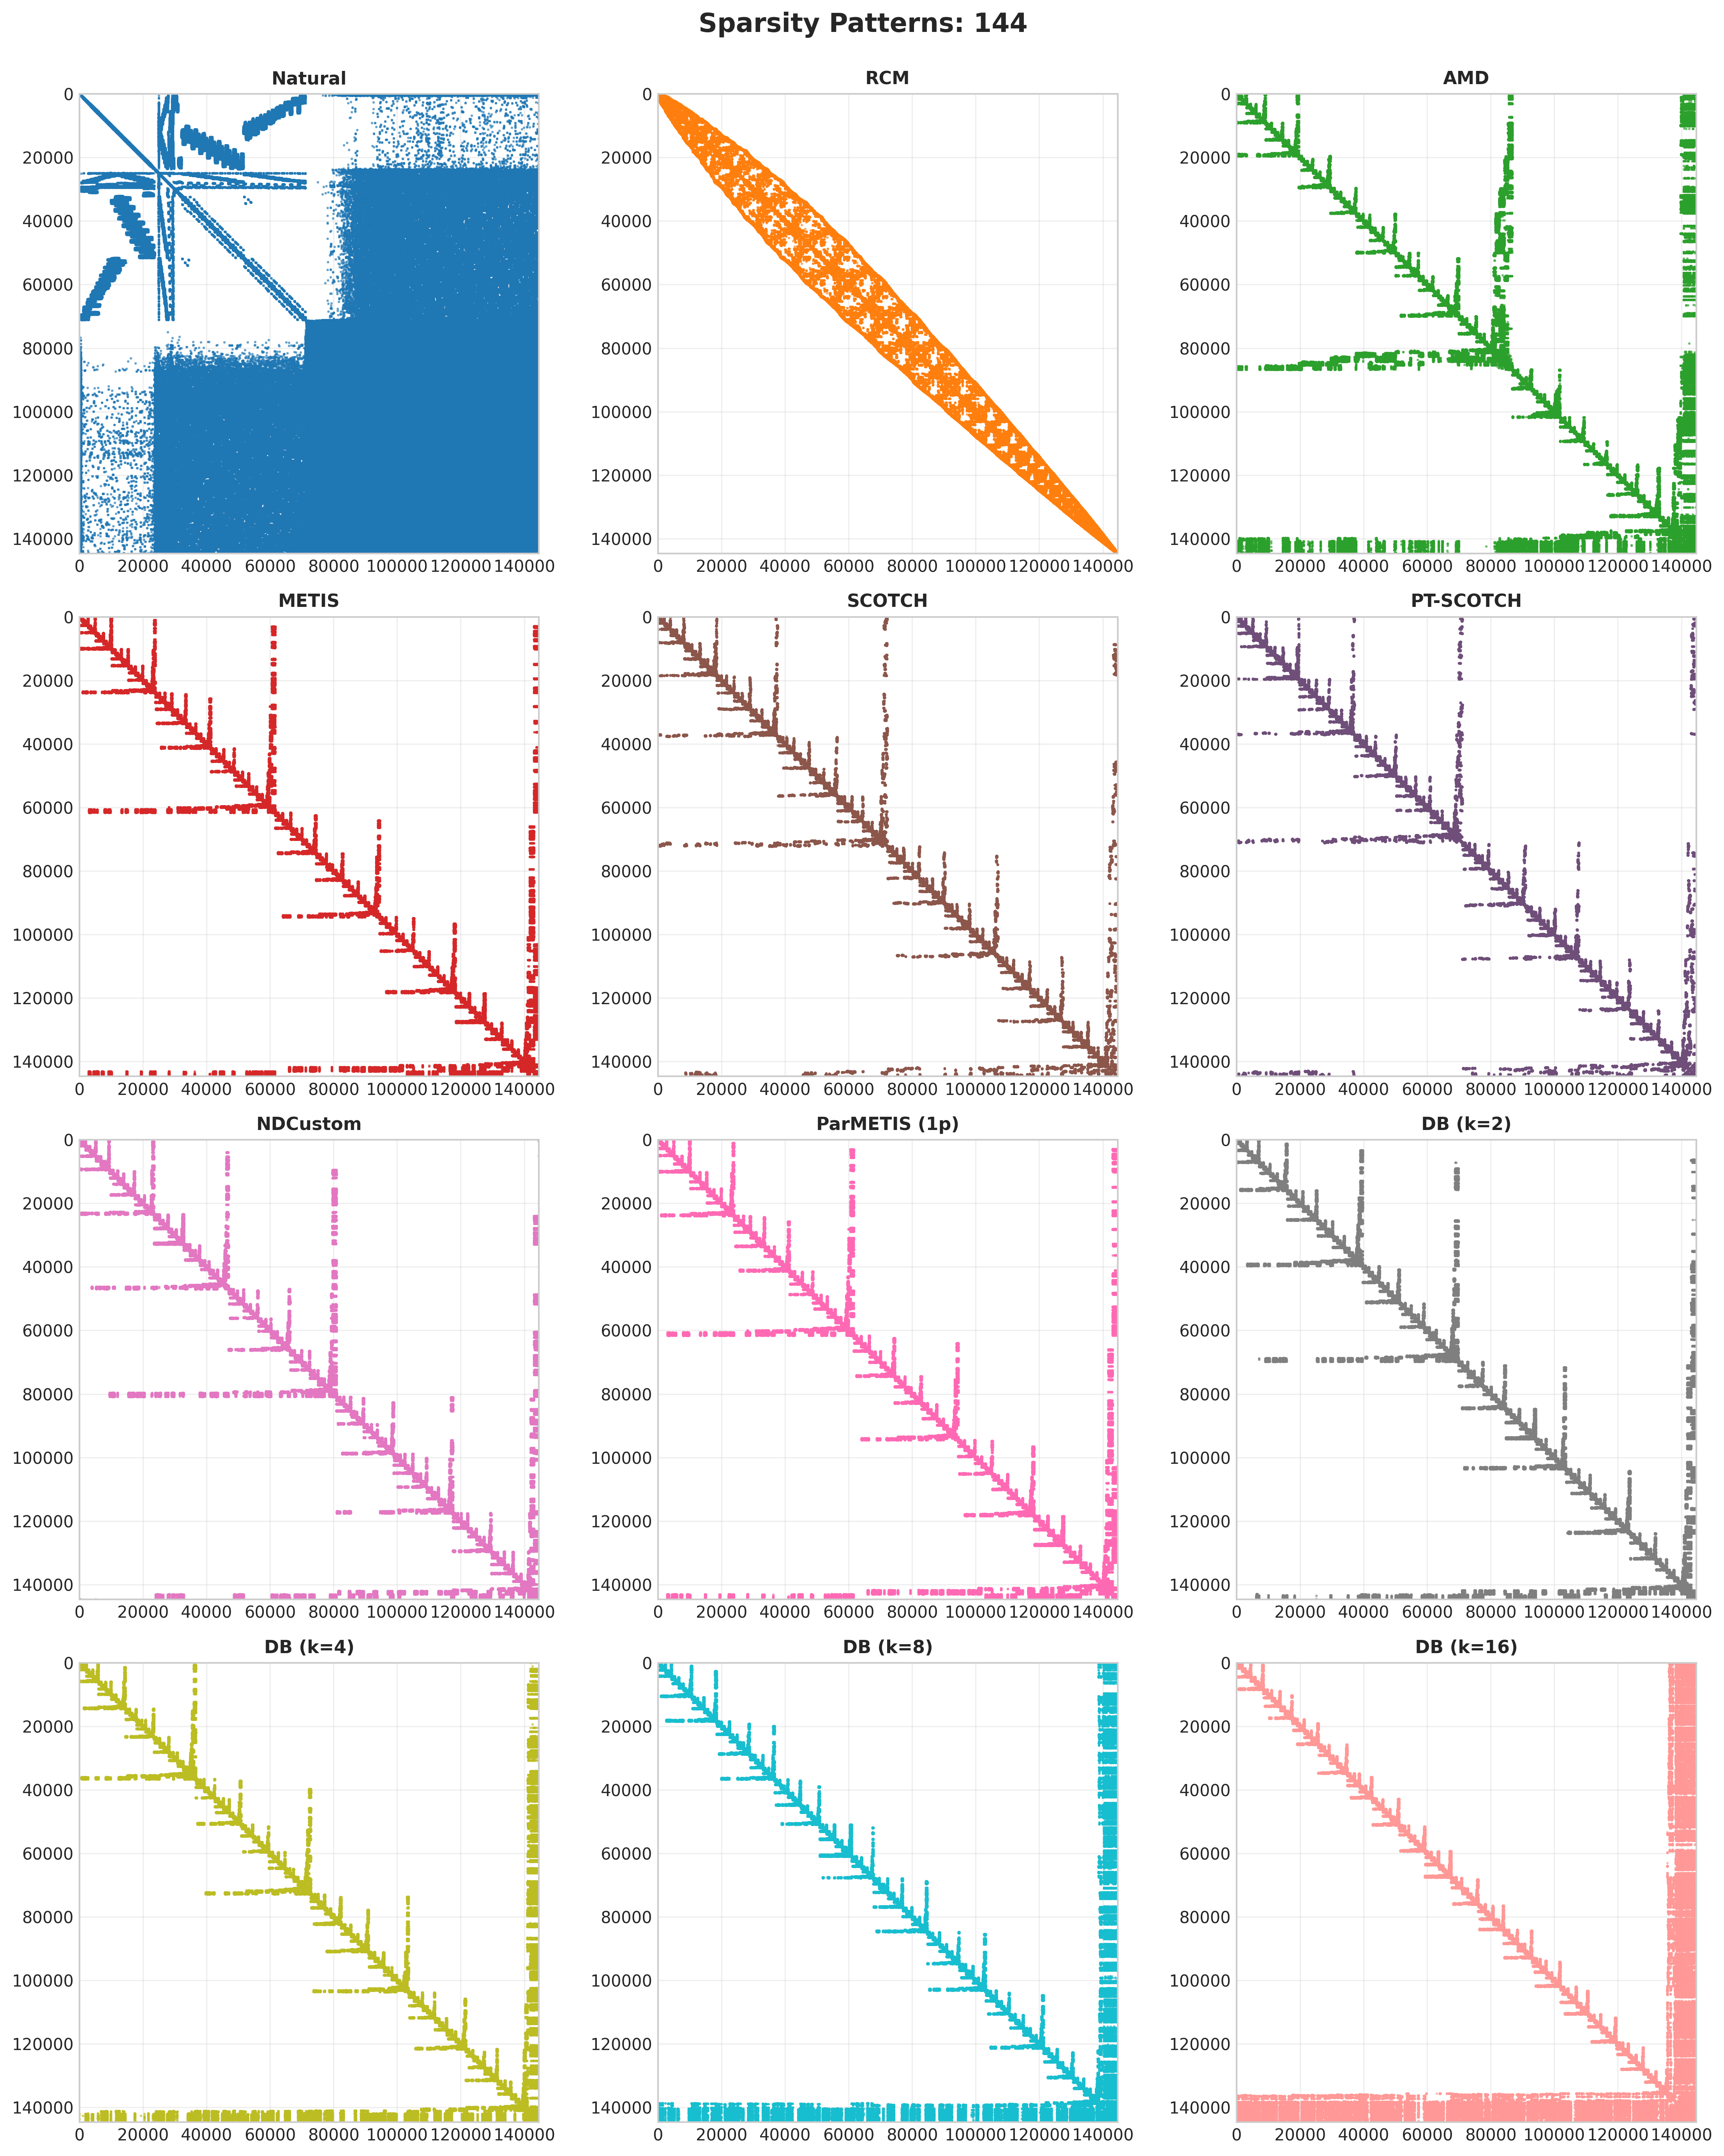
\includegraphics[width=\textwidth]{fig/res/144_sparsity_patterns.png}
\caption{Sparsity patterns of matrix 144 with different reordering algorithms applied. The natural ordering (top-left) shows a scattered pattern leading to high fill-in, while optimized reorderings (other panels) demonstrate more defined structures.}
\label{fig:144-sparsity-patterns}
\end{figure}

\begin{figure}[h]
\centering
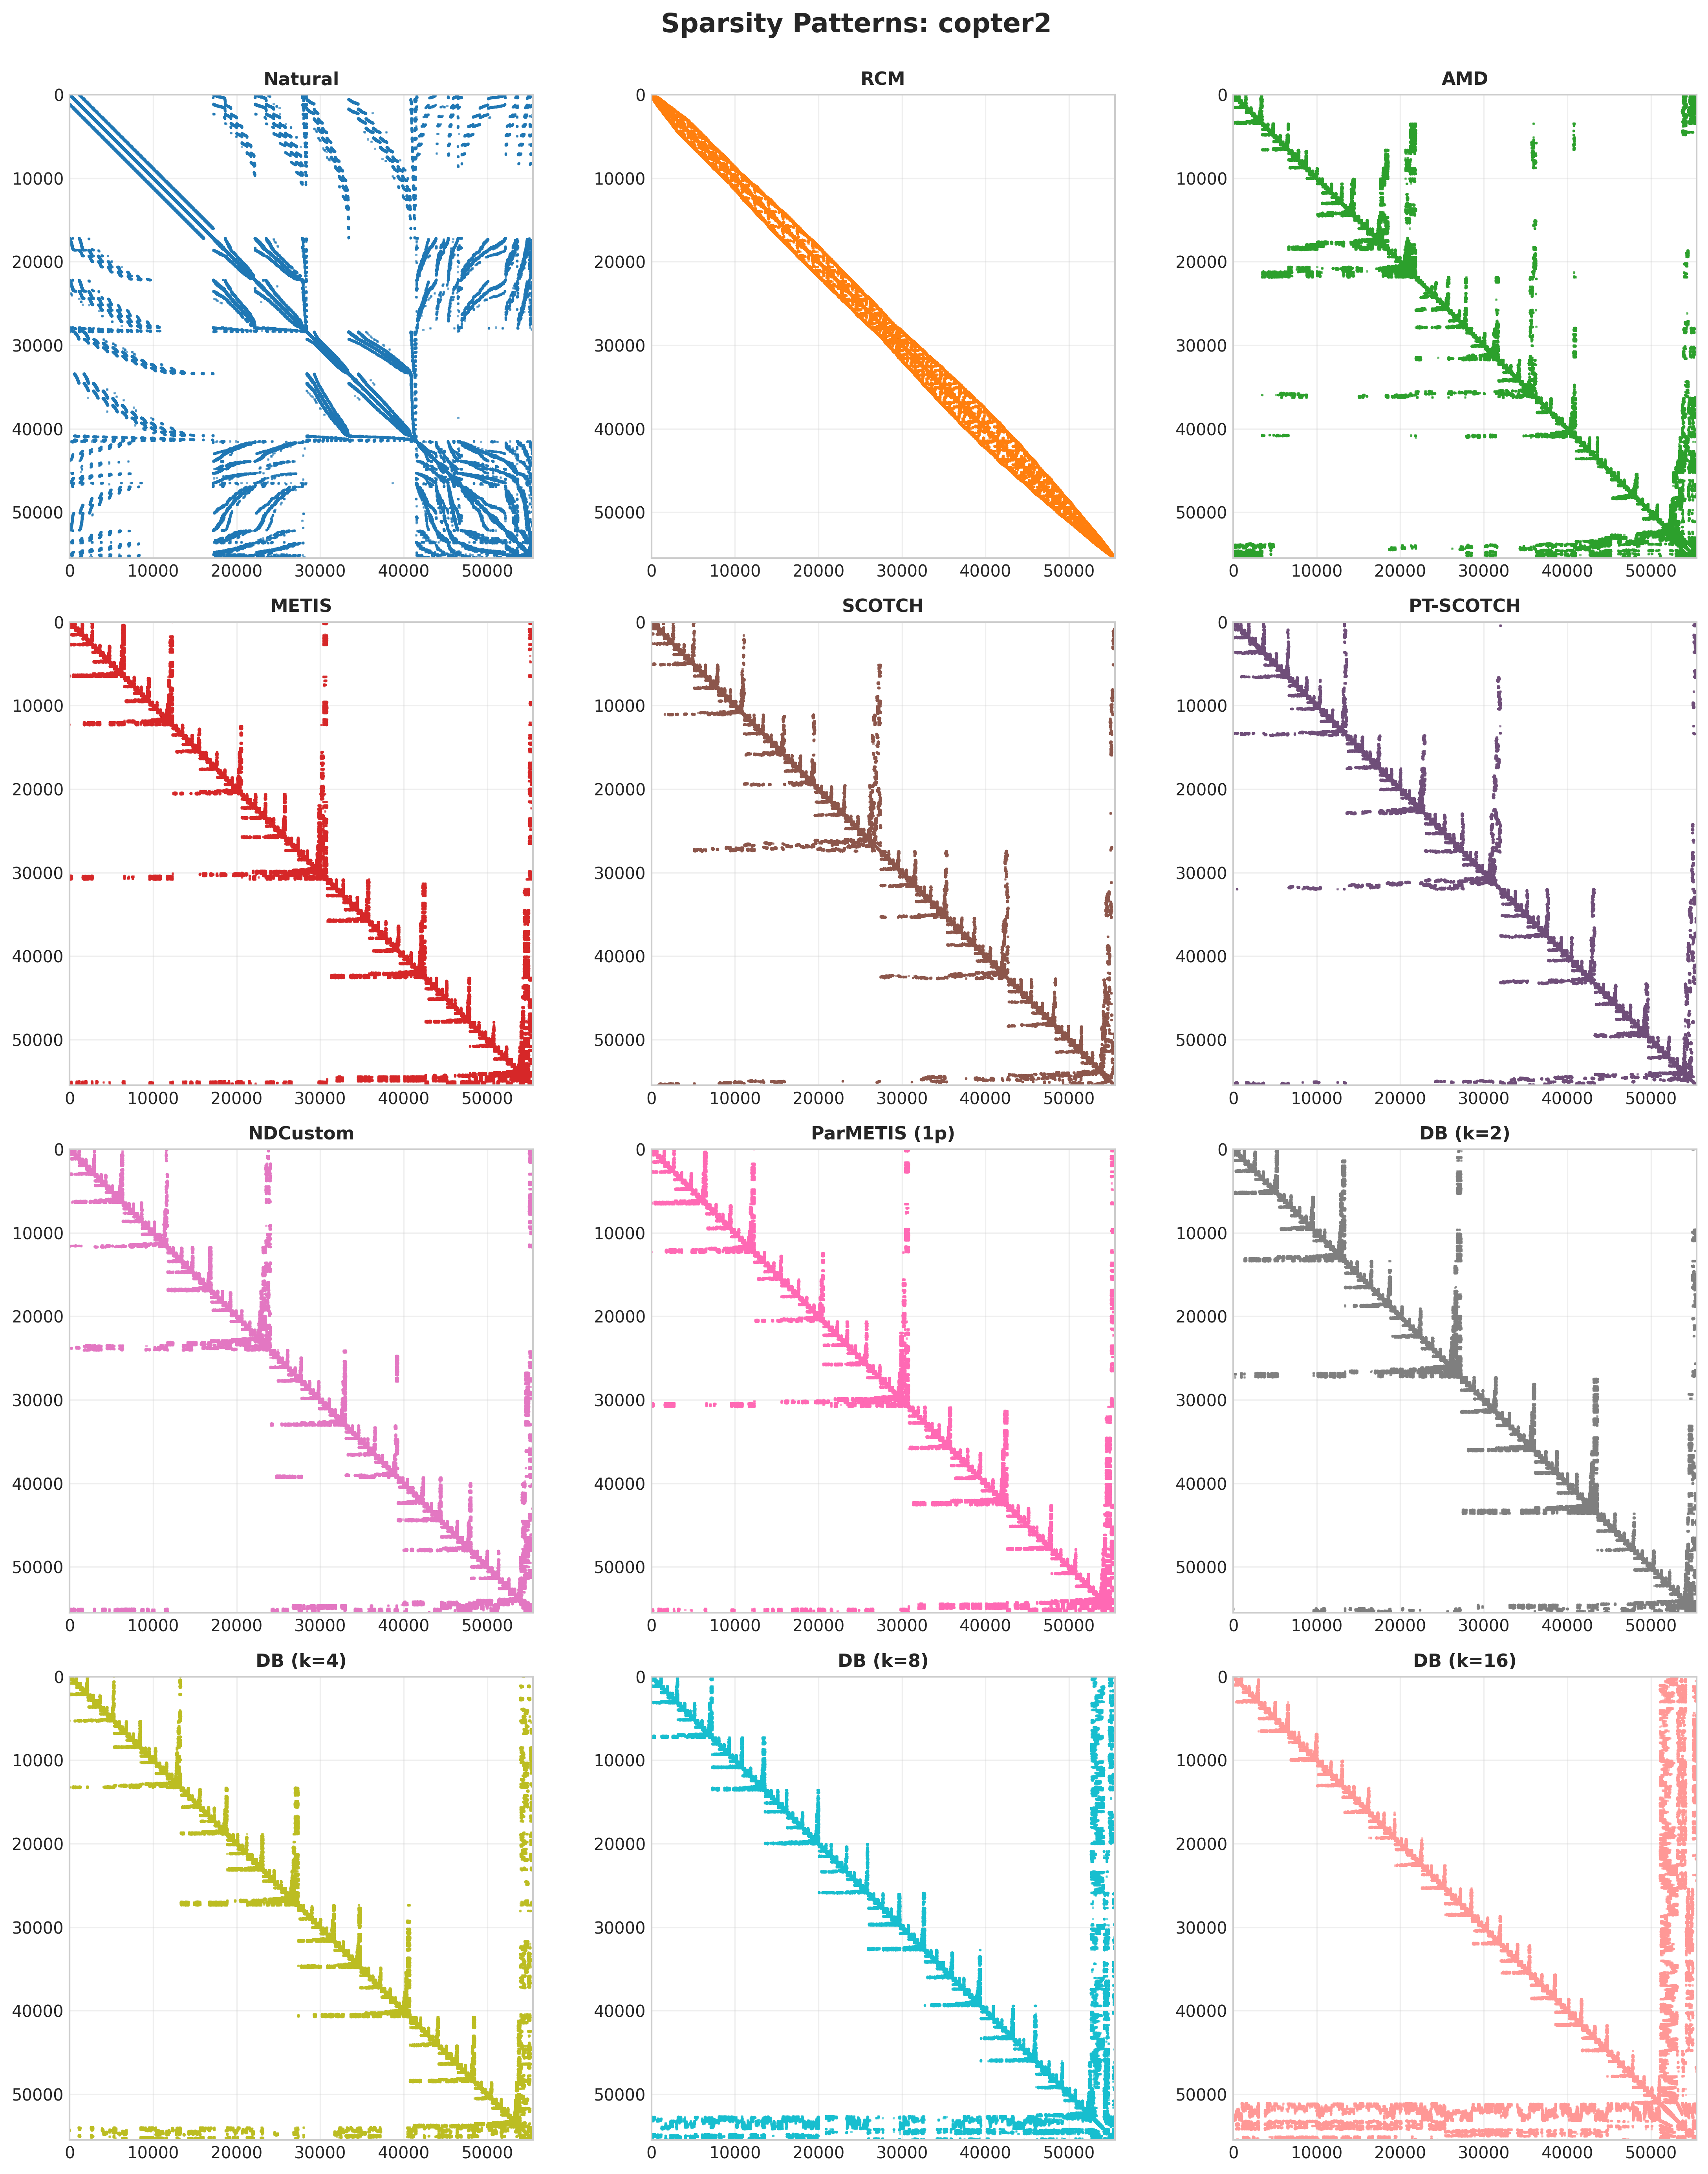
\includegraphics[width=\textwidth]{fig/res/copter2_sparsity_patterns.png}
\caption{Similarly, sparsity patterns of matrix copter2 with different reordering algorithms applied.}
\label{fig:copter2-sparsity-patterns}
\end{figure}



% \section{Current limitations}

% Demonstrating that your implementation meets the objectives is usually done by showing a lower bound on a given figure of merit.
% Conversely, you should also illuminate the limitations of your implementation by showing upper bounds on these (or other appropriate) figures of merit.
% Critically examining your ideas and their implementation trying to find their limits is also part of your work!
